\documentclass[a4paper]{article}

\usepackage[margin=1in]{geometry} 
\usepackage{amsmath,amsthm,amssymb}
\usepackage{float}
\usepackage{graphicx}
\usepackage{xcolor}
\usepackage[UKenglish]{isodate}
\origdate
\cleanlookdateon
\usepackage[hidelinks]{hyperref}
\urlstyle{same}
\usepackage{tocloft}
\renewcommand{\cftsecleader}{\cftdotfill{\cftdotsep}}
\renewcommand{\baselinestretch}{1.25} 
\usepackage{enumitem}
\usepackage{framed}
\usepackage[T1]{fontenc}
\usepackage{kpfonts}
\usepackage{csquotes}
\usepackage{listings}
\usepackage[scaled]{beramono}
\usepackage{lscape}
\usepackage{multirow}
\usepackage{makecell}
\usepackage{graphbox}
\usepackage{pythonhighlight}

\definecolor{eclipseStrings}{RGB}{42,0.0,255}
\definecolor{eclipseKeywords}{RGB}{127,0,85}
\colorlet{numb}{magenta!60!black}

\lstdefinelanguage{json}{
    basicstyle=\normalfont\ttfamily,
    commentstyle=\color{eclipseStrings}, % style of comment
    stringstyle=\color{eclipseKeywords}, % style of strings
    numbers=left,
    numberstyle=\scriptsize,
    stepnumber=1,
    numbersep=8pt,
    showstringspaces=false,
    breaklines=true,
    frame=lines,
    backgroundcolor=\color{white},
    string=[s]{"}{"},
    comment=[l]{:\ "},
    morecomment=[l]{:"},
    literate=
        *{0}{{{\color{numb}0}}}{1}
         {1}{{{\color{numb}1}}}{1}
         {2}{{{\color{numb}2}}}{1}
         {3}{{{\color{numb}3}}}{1}
         {4}{{{\color{numb}4}}}{1}
         {5}{{{\color{numb}5}}}{1}
         {6}{{{\color{numb}6}}}{1}
         {7}{{{\color{numb}7}}}{1}
         {8}{{{\color{numb}8}}}{1}
         {9}{{{\color{numb}9}}}{1}
}

\begin{document}
\title{Midterms Summary\\[0.1cm]
    \large 50.012 Networks, Elective 2019}
\author{Tey Siew Wen}
\date{06 Feb 2020}

\maketitle

\begin{table}[H]
    \centering
    \begin{tabular}{|l|l|l|}
    \hline
    \multicolumn{1}{|c|}{\textbf{Week}} & \multicolumn{1}{c|}{\textbf{Topic}}                                                                                & \multicolumn{1}{c|}{\textbf{Specific Sections}}                                                                                                           \\ \hline
    1 -- 2                                 & Internet Network, Application Layer                                                                                & \begin{tabular}[c]{@{}l@{}}Lecture 1: Transport Layer,\\ Lecture 2: HTTP,\\ Lecture 3: WebAPI\end{tabular}                                                \\ \hline
    3                                   & Multimedia Networking and CDN                                                                                      & \begin{tabular}[c]{@{}l@{}}Lecture 5: Network Applications,\\ Lecture 6: CDN and PNP\end{tabular}                                                         \\ \hline
    4 -- 5                                 & \begin{tabular}[c]{@{}l@{}}Transport Layer Principles\\ Reliable Data Transfer and Congestion Control\end{tabular} & \begin{tabular}[c]{@{}l@{}}Lecture 7: RDT,\\ Lecture 8: RDT Pipelines,\\ Lecture 9: TCP and RDT Principles,\\ Lecture 10: Congestion Control\end{tabular} \\ \hline
    6                                   & TCP                                                                                                                & Lecture 11: TCP Wrapup                                                                                                                                   \\ \hline
    \end{tabular}
    \end{table}

\subsection*{Resources for practice}
Problem sets: \url{http://gaia.cs.umass.edu/kurose_ross/interactive/index.php}

\section*{Learning Checklist}
\subsection*{Week 1 -- 2: Internet Overview and Application Layer}

\noindent\textbf{Overview}
\begin{itemize}[label=$\square$]
    \item Internet Structure: ISPs
    \item The Internet Protocol Stack: APTNLP
    \item Network Performance: Throughput, Delay and Loss Probability
    \item 4 Sources of Packet Delay
    \item Space-Time Diagrams
    \item Circuit Switching vs. Packet Switching
\end{itemize}

\newpage
\noindent\textbf{Application Layer}
\begin{itemize}[label=$\square$]
    \item Application Architectures
    \item Process Communication
    \begin{itemize}[label=$\square$]
        \item Addressing processes with \textit{identifiers}
        \item What are Sockets
    \end{itemize}
    \item Internet Transport Protocol Services: TCP vs. UDP
    \begin{itemize}[label=$\square$]
        \item Socket Programming: Establishment and Usage
        \item Protocol definitions
    \end{itemize}
    \item Electronic Mail Application Protocols
    \begin{itemize}[label=$\square$]
        \item SMTP Interaction and DATA Format
    \end{itemize}
    \item HTTP
    \begin{itemize}[label=$\square$]
        \item Web API
        \begin{itemize}[label=$\square$]
            \item URI, URL, URNs
            \item Architectural Style: REST
        \end{itemize}
        \item Idempotence and safe methods
    \end{itemize}
\end{itemize}

\subsection*{Week 3: Multimedia Networking}

\begin{itemize}[label=$\square$]
    \item Streaming Stored Media
    \begin{itemize}[label=$\square$]
        \item Role of UDP
        \item DASH: Dynamic Adaptive Streaming over HTTP
        \item Interpreting plots for data transmission and playout rate
    \end{itemize}
    \item VoIP (Voice-over-IP)
    \begin{itemize}[label=$\square$]
        \item Adaptive Playout Delay: Average Estimate of Packet Delay, Average Deviation of Delay, Playout time for packets in talk spurts
        \item Recovery From Packet Loss: Simple Forward Error Correction (FEC)    
    \end{itemize}
    \item Streaming Live Media
    \item Content Distribution Networks (CDN) and concerns of CDN Operators
    \begin{itemize}[label=$\square$]
        \item CDN Server Placement
        \item CDN Server Selection
        \item CDN Content Routing
        \item CDN Content Replication
    \end{itemize}
\end{itemize}

\newpage
\subsection*{Week 4: Transport Layer}

\begin{itemize}[label=$\square$]
    \item Multiplexing/Demultiplexing
    \item UDP
    \item Reliable Data Transfer
    \item Flow Control
    \item Congestion Control
    \item TCP Connection Management
\end{itemize}

\newpage
\section{Lecture 1: Transport Layer}
\noindent\textbf{Transport service requirements}
\begin{itemize}
    \item Data loss
    \item Throughput
    \item Time sensitivity
\end{itemize}

\subsection{Protocols}
\subsubsection{TCP/UDP}
\begin{table}[H]
    \centering
    \begin{tabular}{|l|l|}
    \hline
    \multicolumn{1}{|c|}{\textbf{TCP}}                          & \multicolumn{1}{c|}{\textbf{UDP}}                                                                     \\ \hline
    Reliable transport                                          & \begin{tabular}[c]{@{}l@{}}Unreliable data transfer between \\ sending/receiving process\end{tabular} \\ \hline
    \textbf{Flow control:} sender won't overwhelm receiver               & NIL                                                                                                   \\ \hline
    \textbf{Congestion control:} throttle sender when network overloaded & NIL                                                                                                   \\ \hline
    \textbf{Connection-oriented:} setup required between client/server   & No need                                                                                               \\ \hline
    \end{tabular}
\end{table}

For both TCP \& UDP, there is no encryption of data. Hence we have SSL (Secure Sockets Layer)/ TLS (Transport Layer Security) for providing an encrypted TCP connection, ensuring data integrity and end-point authentication. Apps can use SSL/ TLS APIs to do so.

\subsection{Client-server Architecture}
Server is always on with permanent IP address. Hosted in data centers for scaling. Clients communicate with the server and may be intermittently (irregularly) connected with the server. Could have dynamic IP addresses. Clients usually do not communicate directly with each other.

\subsection{Peer-to-peer Architecture}
\begin{itemize}
    \item Server is not always on
    \item Arbitrary End Systems directly communicate: Good for file sharing, overlay-routing
    \item Principles:
    \begin{itemize}[label=$\circ$]
        \item Fault-tolerant
        \item Fate-sharing: It's okay to fail if it's your own mistake?
    \end{itemize}
    \item Self Scalability
    \begin{itemize}[label=$\circ$]
        \item Peers request service from other peers and provide service in return
        \item New peers bring new service capacity and new service demands
    \end{itemize}
    \item Challenges:
    \begin{itemize}[label=$\circ$]
        \item Peers are intermittently connected and change IP addresses
        \item Chunk Poisoning
    \end{itemize}
\end{itemize}

\subsection{Electronic Mail}
3 major components:
\begin{enumerate}
    \item User Agents
    \item Mail Servers
    \begin{enumerate}[label=\roman*.]
        \item Mailbox: contain incoming messages for user
        \item Message Queue: Messages to be sent (outgoing) 
    \end{enumerate}
    \item Simple Mail Transfer Protocol: SMTP
    \begin{itemize}[label=$\circ$]
        \item uses TCP for sending emails from client to server via port 25
        \item has 3 phases of transfer: handshake, transfer, closure.
        \item Requires message to be in 7-bit ASCII
        \item Uses CRLF.CRLF for determining end of message
    \end{itemize}
\end{enumerate}

\noindent Compared to HTTP, SMTP is a push rather than a pull server. Both have ASCII command/res\\ interaction, status codes.

\medskip

\noindent User Agent $\rightarrow$ SMTP $\rightarrow$ Sender Mail Server $\rightarrow$ SMTP $\rightarrow$ Receiver's Mail Server $\rightarrow$ Mail Access Protocol \\$\rightarrow$ User Agent

\medskip

\noindent Mail server: forward mail from sender to receiver mail server. If both the client and the receiver mail server are offline, the sender's mail server will keep retrying to send the mail until it works. Back then the mail servers are not so reliable to on all the time.

\subsubsection{Mail Access Protocol}
Mail Access Protocol is used for retrieval from server
\begin{itemize}
    \item POP (Post Office Protocol)
    \item IMAP (Internet Mail Access Protocol)
    \item HTTPs
\end{itemize}

\subsection{Processes}
Definition of a Process: A program running within the host. It must have an identifier that includes IP address, port numbers associated with the process on host. e.g. HTTP: 80, Mail: 25

\medskip

\noindent Types of Process Communication
\begin{itemize}
    \item Inter-process communication: Dependent on OS
    \begin{itemize}[label=$\circ$]
        \item unless the process is on the application layer, then it is controlled by the app developer.
    \end{itemize}
    \item Host-to-host communication: Exchange Messages
    \begin{itemize}[label=$\circ$]
        \item Messages are sent/received via sockets.
    \end{itemize}
\end{itemize}

\noindent Types of Processes
\begin{itemize}
    \item Client Process: Initiate Communication
    \item Server Process: Waits to be contacted
\end{itemize}

\subsection{Message Segmentation}
\begin{itemize}
    \item Reducing end-to-end delay.
    \item More efficient recovery from bit error. Otherwise the whole message needs to be retransmitted.
    \item Huge message may block other smaller packets
    \item Header overhead linear to the no. of packets
    \item Cause new problems e.g. out-of-order arrival of packets
    \end{itemize}

\newpage
\section{Lecture 2: HTTP}
Each HTTP message designed to be \textit{self-contained}:
\begin{itemize}
    \item it bring as much detail as the server needs to serve that request
    \item server does not maintain state
\end{itemize}
\textbf{Protocols that maintain state} are complex
\begin{itemize}
    \item Past History must be maintained
    \item If server/client crash, the state that is stored on either host will be inconsistent
    \item however doing so is likely to improve performance
\end{itemize}

\subsection{HTTP Methods}
\textbf{\textit{Safe Methods}} e.g. GET, HEAD:
\begin{itemize}
    \item enable caching and loading distribution
    \item does not modify resources on server
\end{itemize}
\textbf{\textit{Idempotent}} Methods e.g. Multiple DELETE:
\begin{itemize}
    \item \textit{Definition}: An effort that can be applied multiple times without changing the result beyond the initial application.
    \begin{itemize}[label=$\circ$]
        \item Handle lost confirmations by re-sending
        \item May modify resources on the server
        \item Can be executed multiple times without changing outcome
        \end{itemize}
    \item Counter e.g. Multiple POST
\end{itemize}

\subsection{Proxy}
\textit{Definition}: An entity authorized to act on behalf of another e.g. an intermediatory server performing requests for us
\begin{itemize}
    \item Serve as a single point access of control to enforce security protocols
\end{itemize}

\noindent\textbf{Common traits of proxies}:
\begin{itemize}
    \item Single access of control
    \item Load Balancing: Distribute incoming requests to a cluster of servers, all provide the same kind of service
\end{itemize}

\subsubsection{Forward Proxy}
When a client makes a connection attempt to that file transfer server on the Internet, its requests usually have to \textit{pass through the forward proxy first}, where a firewall will be behind it.
\begin{enumerate}
    \item Depending on the forward proxy's settings, a request can be allowed or denied.
    \item If allowed, then the request is forwarded to the firewall and then to the file transfer server.
    \item From the point of view of the file transfer server, it is the proxy server that issued the request, not the client. So when the server responds, it addresses its response to the proxy.
    \item When the forward proxy receives the response, it recognizes it as a response to the request that went through earlier. And so it in turn sends that response to the client that made the request.
\end{enumerate}

\noindent Applications:
\begin{itemize}
    \item Content Logging \& Eavesdropping
    \item Accessing Services Anonymously
\end{itemize}

\subsubsection{Reverse Proxies}
The reverse proxy does the exact opposite of what a forward proxy does. It accepts requests from external clients on behalf of servers stationed behind it. The firewall is between the client and reverse proxy instead of being in between the forward proxy and the servers.

\begin{enumerate}
    \item Depending on the reverse proxy's settings, a request can be allowed or denied.
    \item From the perspective of the client, it is the reverse proxy that is providing file transfer services.
\end{enumerate}

\noindent Applications:
\begin{itemize}
    \item A/B testing, Multivariate testing
    \item Distribute load
\end{itemize}

\newpage
\section{Lecture 3: Web API}
Application programming interface (API) specifies how 2 software components should interact.

\subsection*{Types of API Protocols}
\subsection{Simple Object Access Protocol (SOAP)}
Simple Object Access Protocol (SOAP) is the specific protocol for XML-based data exchange, popular in enterprise M-M communication.
\begin{itemize}
    \item However, specific protocols seem to add overhead in many cases.
\end{itemize}
Web service definition language (WSDL) is used to specify the available services to clients.
\begin{itemize}
    \item Client-side functions to call API can be automatically generated
    \item Auto-completion for API calls
\end{itemize}

\subsection{Representational State Transfer (REST)}
Representational State Transfer (REST) is not a protocol, but rather an architectural style.

\begin{itemize}
    \item Pros: Simple, scalable, general, high performance
    \item Cons: No-built-in ACID \& Under-fetching/Over-fetching
    \begin{itemize}[label=$\circ$]
        \item ACID: Atomicity, Consistency, Isolation, Durability
        \item Over-fetching: You might get more data than you need, but the end point is designed to give you that specific data.
        \item Underfetching: You might get less data than you need, because there is no end point designed to give you the data you need from that server.
    \end{itemize}
\end{itemize}

\subsubsection{Resources in REST}
\begin{itemize}
    \item Types
    \begin{enumerate}[label=\roman*.]
        \item Collections
        \item Instances
    \end{enumerate}
    \item Referenced in the HTTP header
\end{itemize}

\begin{table}[H]
    \centering
    \begin{tabular}{|l|l|}
    \hline
    \multicolumn{1}{|c|}{\textbf{Simple Static Settings}} & \multicolumn{1}{c|}{\textbf{Dynamic Settings}}                                                                                                                                             \\ \hline
    Each resource corresponds to single file.             & \begin{tabular}[c]{@{}l@{}}Server will interpret the URL as parameters,\\ dynamically create content for provided parameters.\\ \\ Content at resource URL may not exist yet.\end{tabular} \\ \hline
    \end{tabular}
\end{table}

\subsubsection{Running HTTP Requests with curl}
At any point of time, if you want to understand more about the flags that you pass into curl to test your http requests, run \texttt{curl --help}. Examples of sending a get request and giving the \texttt{-v} flag to show more information on exchanged messages. For a patch request, you can run:
\texttt{curl -H "Content-Type: application/json" -X PATCH -d '{"title":"test"}' http://jsonplaceholder.typicode.com/todos/199}
\newpage
\noindent The result will be:
\begin{lstlisting}[language=json,firstnumber=1]
    {
        "userId": 10,
        "id": 199,
        "title": "test",
        "completed": true
    }
\end{lstlisting}

\paragraph{PUT vs POST}
\begin{itemize}
    \item PUT: Used to update an existing resource. Reply will be 200. 
    \item POST: Used to create an element in a collection. Reply will be 201 with URL of created element.
\end{itemize}

\subsection{Multipurpose Internet Mail Extensions (MIME)}
Multipurpose Internet Mail Extensions (MIME) is an Internet standard that extends the format of email messages to support text in character sets other than ASCII, as well attachments of audio, video, images, and application programs. Message bodies may consist of multiple parts, and header information may be specified in non-ASCII character sets.

\section{Lecture 5: Network Applications}
\subsection{Streaming stored video}
\begin{itemize}
    \item Use Redundancy within and between images to decrease \# bits required to encode image
    \begin{itemize}[label=$\circ$]
        \item Spatial (within image)
        \item Temporal (from one image to next)
    \end{itemize}
    \item Encoding Rate
    \begin{itemize}[label=$\circ$]
        \item CBR (Constant Bit Rate): Fixed encoding rate
        \item VBR (Variable Bit Rate): Changes as amount of spatial, temporal coding changes
    \end{itemize}
    \item Challenges
    \begin{itemize}[label=$\circ$]
        \item Continuous playout constraint: Once client playout begins, playback must match original timing
        \begin{itemize}[label=\tiny$\blacksquare$]
            \item Network Delay e.g. queue delay are variable $\rightarrow$ need client side buffer to match playout requirements
        \end{itemize}
        \item Client Interactivity: Allow pause, fast-forward, rewind and jump through video
        \item Video packets may be lost, need to retransmit    
        \begin{itemize}[label=\tiny$\blacksquare$]
            \item Packets may be received slower than it is being sent, so some packets might be skipped.
        \end{itemize}
    \end{itemize}
\end{itemize}

\newpage
\subsubsection{Streaming multimedia: DASH}
DASH stands for Dynamic, Adaptive Streaming over HTTP (DASH).

\bigskip

\noindent Other adaptive solutions: Apple's HTTP Live Streaming (HLS) solution, Adobe Systems HTTP Dynamic Streaming, Microsoft Smooth Streaming
\begin{itemize}
    \item Server
    \begin{itemize}[label=$\circ$]
        \item encodes video file into multiple versions
        \item each version stored, encoded at a different rate
        \item manifest file: provide URLs for different versions
        \end{itemize}
    \item Client
    \begin{itemize}[label=$\circ$]
        \item Handles most of the streaming logic:
        \begin{itemize}[label=\tiny$\blacksquare$]
            \item When to request chunk
            \item What encoding rate to request
            \item Where to request
        \end{itemize}
    \end{itemize}
\end{itemize}

\subsection{Voice over IP (VoIP)}
VoIP end-end-delay requirement: <150 ms good, >400ms bad

\begin{itemize}
    \item For delay jitter, we aim to minimize client playout delay
    \item Receiver attempts to playout each chunk exactly q msecs after chunk is generated
    \begin{itemize}[label=$\circ$]
        \item Large q: less packet loss
        \item Small q: better interactive experience
    \end{itemize}
\end{itemize}

\subsubsection{Adaptive Playout Delay}
\paragraph{Adaptively Estimate Packet Delay}
\mbox{}
\bigskip

\noindent \underline{Exponentially Weighted Moving Average (EWMA)}
\begin{align*}
    d_i = (1-\alpha)d_{i-1} + \alpha(r_i - t_i)
\end{align*}
where:
\begin{itemize}
    \item $d_i$ is the delay estimate after $i$-th packet
    \item $\alpha$ is a small constat
    \item $r_i$ is the time received, $t_i$ is the time sent
    \item so $r_i - t_i$ is the measured delay of $i$-th packet
    \end{itemize}

\bigskip

\noindent \underline{Average deviation of delay}
\begin{align*}
    v_i = (1-B)v_{i-1}+B|r_i-t_i-d_i|
\end{align*}
$d_i$, $v_i$ are calculated for every received packet, but used only at the start of talk spurt.
\begin{itemize}
    \item 1st packet in talkspurt: $ \text{playout}-\text{time}_i = t_i + d_i + Kv_i$
    \begin{itemize}[label=$\circ$]
        \item longer playback delay
    \end{itemize}
    \item Remaining packets are played out periodically
\end{itemize}

\newpage
\section{Lecture 6: CDN and PNP}
\subsection{Content Distribution Networks (CDN)}
Problem Background: Streaming Content to hundred of thousands of simultaneous users

\bigskip

\noindent Possible solutions:
\begin{enumerate}
    \item Single mega server: doesn't scale
    \begin{itemize}[label=$\circ$]
        \item point of network congestion
        \item long path to distant clients
        \item single point of failure
        \item multiple copies of vid sent over outgoing link
    \end{itemize}
    \item Store/serve multiple copies of videos at multiple geographically distributed sites (CDN)
\end{enumerate}
CDN Operators stores copies of content at CDN Nodes.

\subsubsection{CDN Server}
\paragraph{Types of CDN}
\begin{itemize}
    \item Commercial CDN: e.g. Akamai, Cloudflare
    \item Content provider's own CDN: e.g. Google, netflix
    \item Telco CDN
\end{itemize}

\paragraph{Choice of Placement}
\begin{itemize}
    \item Push CDN servers deep into many access ISPs so that they are close to users
    \item Smaller no. of larger clusters in IXPs near access ISPs
\end{itemize}

\paragraph{Server Selection}\mbox{}

\medskip
\noindent Points of consideration:
\begin{itemize}
    \item Geographically close
    \item Performance: Real-time measurement
    \item Load-balancing
    \item Cost: CDN may need to pay its provider ISP
    \item Fault-tolerance
\end{itemize}

\paragraph{Routing the Content}\mbox{}

\medskip
\noindent After selection, we still have a routing problem. We can route content access in 3 different ways:
\begin{enumerate}
    \item DNS-based
    \item Application Driven
    \begin{itemize}
        \item Multiple connection setup, name lookups
    \end{itemize}
    \item Routing (anycast)-based
\end{enumerate}

\paragraph{Content Replication}\mbox{}

\medskip
\noindent Mechanisms:
\begin{itemize}
    \item Push: Use of off-peak bandwidth optimization
    \item Pull: More Adapative
\end{itemize}
\noindent e.g. Netflix
\begin{itemize}
    \item has prepared content
    \item so push content to CDN during off-peak hours whose CDN servers pull \& cache content by user demand.
\end{itemize}
\noindent e.g. Youtube
\begin{itemize}
    \item people can upload content anytime
    \item so CDN servers pull content by user demand at all time
\end{itemize}

\subsection{Peer-to-peer architecture}
\begin{itemize}
    \item Arbitrary end systems directly communicate as peers
    \item Peers are intermittently connected and may change IP addresses
\end{itemize}
e.g. VoIP (Skype), Multimedia Streaming (Kankan.com), File Distribution (BitTorrent)

\subsubsection{File distribution time (lower bound)}
\begin{itemize}
    \item $d_{min}$: min client download rate
    \item $\displaystyle\frac{F}{d_{min}}$: min client download time
    \item $\displaystyle\frac{F}{u_s}$: server upload time for one copy of file
\end{itemize}

\paragraph{Client-server}
\begin{itemize}
    \item Server must sequentially upload N file copies (to N clients)
    \item Each client must download file copy
\end{itemize}
\textbf{Time to distribute F to N clients:} $$ D_{c-s} \geq \max\left(N\frac{F}{u_s}, \frac{F}{d_{min}}\right)$$

\paragraph{P2P}
\begin{itemize}
    \item Server must upload at least one copy
    \item Each client must download one file copy
    \item Clients as aggregate must download $NF$ bits
\end{itemize}
\textbf{Time to distribute F to N clients} $$ D_{p2p} \geq \max\left(\frac{F}{u_s},\frac{F}{d_{min}}, N\frac{F}{u_s+\sum{u_i}}\right) $$
Another simplification of the third term of the equation: $$N\frac{F}{u_s+\sum{u_i}} = \frac{F}{u_s/N+u} $$

\section{Lecture 7: Reliable Data Transport}
\subsection{Principles of Reliable Data Transport}
\begin{enumerate}
    \item Physical channels are never completely reliable
    \begin{itemize}[label=$\circ$]
        \item Wireless links subjected to interference
        \item Transmission noise $\rightarrow$ lead to bit errors
        \item Routers \& Switches may drop packets due to buffer overflow
    \end{itemize}
    \item Reliable communication relies on \textbf{detection and retransmissions as necessary}.
    \begin{itemize}[label=$\circ$]
        \item Receiver: Acknowledges packets from the sender.
        \item Sender: Transmits \& retransmits based on information provided by the receiver. If the sender times out (ack/nack not received within a certain time-frame). An action will be triggered.
        \item Packets: Contain \hyperref[seqnum]{\textcolor{blue}{sequence numbers}}
    \end{itemize}
\end{enumerate}

\subsubsection{Model for Reliable Communication}
\begin{itemize}
    \item Provides send/receive methods for applications to transfer packets
    \item Fields in packet header is used to coordinate with peer
\end{itemize}

\subsection{Basic RDT Protocols}
\begin{itemize}
    \item RDT 1.0: Assume reliable channel
    \item RDT 2.0: Considers that channel may be corrupted.
    \item RDT 2.1: RDT 2.0 + 1-bit \texttt{seq\_num} for identifying packet loss.
    \item RDT 2.2: RDT 2.1 + Stop and wait.
    \item RDT 3.0: RDT 2.2 + timeouts
\end{itemize}

\subsubsection{RDT 2.0 \& 2.1}
\underline{Assumptions}
\begin{enumerate}
    \item Channel may corrupt but never lose packets.
    \begin{itemize}[label=$\circ$]
        \item Receiver always get something whenever a packet is sent
        \item Sender always receives an ack after sending a packet (Feedback)
    \end{itemize}
    \item Receiver can always detect if packet has been corrupted.
    \begin{itemize}[label=$\circ$]
        \item Checksum to detect bit errors
        \begin{itemize}[label=\tiny$\blacksquare$]
            \item May be flawed as the checksum could still tally after modification to data
        \end{itemize}
    \end{itemize}
\end{enumerate}

\noindent \underline{Communication Flow}
\begin{itemize}
    \item Sender: Transmits one packet at a time and waits for ack/nack
    \item Receiver: Sends ack when it receives packet correctly, and sends nack when it receives erroneous packet.
\end{itemize}

\newpage
\noindent \underline{Challenges}
\begin{itemize}
    \item Corruption: The reality is that packets, acks, nacks can all get corrupted.
    \begin{itemize}[label=$\circ$]
        \item This means that the sender may not be able to tell which packet was received correctly or not.
        \item If sender retransmits the packet, the receiver could deliver the same packet to the application twice. If it transmits a new one, the receiver can fail to deliver a packet to the application.
    \end{itemize}
    \item Lost Packets
    \begin{itemize}[label=$\circ$]
        \item Receiver does not know that a packet was sent to it, so it won't send an ack response
        \item Sender left waiting for ack, but ack never comes :(
    \end{itemize}
\end{itemize}

Hence the 1-bit \texttt{seq\_num} is introduced in RDT2.2, such that nack is not necessary anymore.

\subsubsection{RDT 2.2}
Stop and wait (Alternating-bit protocol)
\begin{itemize}
    \item Sender sends one packet and waits for receiver response
\end{itemize}

\paragraph{Importance of Sequence Numbers (\texttt{seq\_num})}
\label{seqnum}
\begin{itemize}
    \item \texttt{seq\_num} in ack identifies received packet(s)
    \item Size of \texttt{seq\_num}: Determines num of packets that can be sent before acknowledgements must be received
\end{itemize}

\begin{table}[H]
    \centering
    \begin{tabular}{|l|l|}
    \hline
    \multicolumn{1}{|c|}{\textbf{Sender}}                                                                   & \multicolumn{1}{c|}{\textbf{Receiver}}                                                                                              \\ \hline
    Adds \texttt{seq\_num} to packet                                                                        & \begin{tabular}[c]{@{}l@{}}Must check if received packet's \texttt{seq\_num} != \\ previously stored \texttt{seq\_num}\end{tabular} \\ \hline
    \begin{tabular}[c]{@{}l@{}}Must check if received ACK matches \\ correct \texttt{seq\_num}\end{tabular} & \begin{tabular}[c]{@{}l@{}}Receiver cannot know if its last ACK \\ received OK at sender\end{tabular}                               \\ \hline
    \end{tabular}
\end{table}

\paragraph{Scenarios}\mbox{}

\medskip
\noindent Case: Corrupted packet
\begin{itemize}
    \item Receiver not receiving pkt1 as intended
\end{itemize}
\begin{figure}[H]
    \centering
    \includegraphics[width=0.2\linewidth]{images/corruptpacket.png}
\end{figure}

\noindent Case: Corrupted ack
\begin{itemize}
    \item Sender not receiving ack0, so it retransmit pkt0
\end{itemize}
Case: Corrupted packet + Corrupted ack
\begin{itemize}
    \item 1st packet and its ack not corrupted
    \item 2nd packet is corrupted so it is sent a 2nd time.
    \item During the 2nd time, the packet is not corrupted but the ack is corrupted
\end{itemize}
\begin{figure}[H]
    \centering
    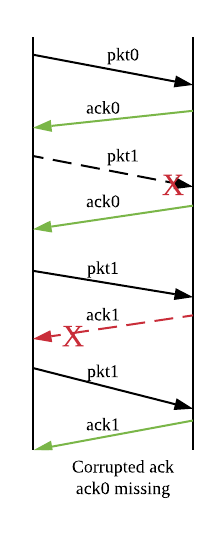
\includegraphics[width=0.2\linewidth]{images/rdt_noack3.png}
\end{figure}

\subsubsection{RDT 3.0}
Previously RDT 2.2 did not address the issue of lost packets. There are a few ways of recovering from lost packets:
\begin{enumerate}
    \item Keep sending packet repeatedly until sender gets an ack
    \begin{itemize}[label=$\circ$]
        \item Sender and receiver both will do extra work
    \end{itemize}
    \item Sender waits for ack for a specified time, then re-sends the packet if ack fails to arrive in time (timeout)
    \begin{itemize}[label=$\circ$]
        \item Works well if maximum ack delay is known and \textbf{does not change}. Otherwise will lead to premature timeout.
    \end{itemize}
\end{enumerate}

\paragraph{Features of RDT 3.0}\mbox{}

\medskip
\noindent \textit{RDT3.0 is the correct way of implemeting RDT but inefficient.}
\begin{itemize}
    \item Involves timeout before retransmission
    \item Sends only 1 packet at a time
    \item works well if delay between sender \& receiver is small
    \item inefficient if $RTT \gg t_{pkt}$ where $t_{pkt}=\displaystyle\frac{L}{C}$
\end{itemize}
\noindent\textit{Example of ineffiency:}\\
Consider a 1 Gb/s link with 10 ms delay in each direction, where RDT 3.0 sends only 1 packet every 20ms. The link is actually capable of sending 20 million bits in 20ms, so for typical packet sizes, only tiny fraction of link's capacity is used.

\paragraph{Calculating the Performance of RDT 3.0}
Important variables
\begin{itemize}
    \item $t_{pkt}=\displaystyle\frac{L}{C}$
    \item $t_{out}$: RTT
    \item ${C}$: link speed
    \item ${L}$: average packet size
    \item ${q}$: packet loss/corruption probability
\end{itemize}
\noindent If given $p$, the time to travel from sender to receiver and $p'$, the time to travel from receiver to sender,
$$ q = p+(1-p)p' $$

\noindent\underline{Expected time between successful transmissions $(T_{succ})$}
\begin{align*}
    T_{succ} &= \sum^\infty_{k=0}(k+1)(RTT+t_{pkt})(q^k)(1-q)(RTT+t_{pkt})\frac{1}{(1-q)^2}\\
    &= \frac{RTT+t_{pkt}}{1-q}
\end{align*}

\noindent\underline{Throughput}
$$\frac{L}{T_{succ}} = C(1-q)\left(1+\frac{RTT}{t_{pkt}}\right)$$
Thoroughput improves if
\begin{itemize}
    \item corruption probabiliy/loss get smaller
    \item RTT gets smaller compared to $t_{pkt}$
\end{itemize}

\noindent\underline{Utilization}

\medskip
\noindent Fraction of time sender is busy sending
$$ U = \frac{D}{RTT+D}$$

\noindent Space-time diagram
\begin{figure}[H]
    \centering
    \includegraphics[width=0.7\linewidth]{images/rdt_stopandwait.PNG}
\end{figure}    

\paragraph{Requirements of Timeout}
$$\text{Timeout} \geq RTT \text{ where } RTT = d_{nodal(data)} + d_{nodal(ack)}$$
Recall that $d_{nodal} = d_{proc} + d_{queue} + d_{trans} + d_{prop}$.

\medskip

\noindent\underline{Challenges}
\begin{itemize}
    \item Premature timeout: sender receives ack late, after it has retransmitted the packet that it did not receive ack for.
    \item Estimating RTT: Components are unknown and variable
\end{itemize}

\subsubsection{Finite State Machine Diagrams}
\begin{table}[H]
    \setcellgapes{5pt}
    \makegapedcells
    \centering
    \begin{tabular}[t]{|c|c|c|}
    \hline
    \textbf{Protocol} & \textbf{Sender} & \textbf{Receiver} \\ \hline
    RDT 2.1           & \includegraphics[width=0.42\linewidth, align=c, trim={1cm 0 0 0}, clip]{images/rdt21_sender.PNG} &\includegraphics[width=0.42\linewidth, align=c]{images/rdt21_receiver.PNG}\\ \hline
    RDT 2.2           & \includegraphics[width=0.42\linewidth, align=c, trim={0.7cm 0 0 0}, clip]{images/rdt22_sender.PNG} &\includegraphics[width=0.42\linewidth, align=c, trim={0.7cm 0 0 0}, clip]{images/rdt22_receiver.PNG}\\ \hline
    RDT 3.0           & \includegraphics[width=0.42\linewidth, align=c, trim={0.7cm 0 0 0}, clip]{images/rdt30_sender.PNG} &\includegraphics[width=0.42\linewidth, align=c]{images/rdt30_receiver.jpg}\\ \hline
    \end{tabular}
\end{table}

\newpage
\section{Lecture 8: RDT Pipelines}
Pipelining allows for increased utilization of the link.
\begin{table}[H]
    \setcellgapes{5pt}
    \centering\makegapedcells
    \begin{tabular}[t]{|c|c|}
    \hline
    \textbf{Without pipeline} & \textbf{With pipeline} \\ \hline
    \includegraphics[width=0.45\linewidth, align=c]{images/rdt30_stopandwait.PNG}&\includegraphics[width=0.45\linewidth, align=c]{images/rdt30_pipeling.PNG}\\ \hline
    \end{tabular}
\end{table}

\subsection{Consequences of pipelining}
\begin{itemize}
    \item The range of \texttt{seq\_num} must be increased, since each in-transit packet must have a unique number and there may be multiple, in-transit, unack packets. (not counting retransmissions)
    \item Minimally, the sender will have to buffer packets that have been transmitted but not ack yet.
\end{itemize}
There are 2 basic approaches towards pipelined error recovery:
\begin{enumerate}
    \item Go-Back-N (GBN): \href{https://media.pearsoncmg.com/aw/ecs_kurose_compnetwork_7/cw/content/interactiveanimations/go-back-n-protocol/index.html}{\textcolor{blue}{Interactive Animation}}
    \item Selective Repeat (SR): \href{https://media.pearsoncmg.com/aw/ecs_kurose_compnetwork_7/cw/content/interactiveanimations/selective-repeat-protocol/index.html}{\textcolor{blue}{Interactive Animation}}
\end{enumerate}

\subsection{Types of Pipeline Protocols}
\subsubsection{Go-Back-N (GBN)}
\textbf{Sender}

\medskip
\noindent The sender is allowed to transmit multiple packets without waiting for an ack, where:
\begin{itemize}
    \item \texttt{N}: the no. unack packets in the pipeline / the window size.
    \item \texttt{base}: the \texttt{seq\_num} of the oldest unack packet.
    \item \texttt{nextseqnum}: smallest unused \texttt{seq\_num}, the index of the next packet to be sent.
    \item \texttt{seq\_num\_space}: range of [$0$, $2^k-1$]
    \item \texttt{seq\_num} with $k$ number of bits for the packet sequence number field in the packet header.
\end{itemize}

\begin{figure}[H]
    \centering
    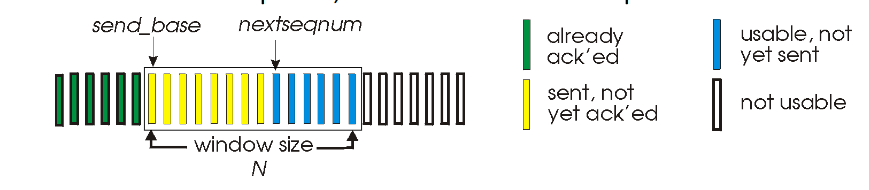
\includegraphics[width=0.7\linewidth]{images/GNB.PNG}
\end{figure}
\newpage
This results in the following array of packets at the sender's side:
\noindent The result will be:
\begin{python}
    data = seq_num_space
    ack_pkts = data[0:base]
    window = data[base:base+N]
    sent_unack_pkts = data[base:nextseqnum]
    avail_pkts_to_send = data[nextseqnum:base+N]
    outside_window = data[base+N::]
\end{python}
As such, it is referred to the \textbf{sliding-window protocol}.
\bigskip

\noindent \textbf{Receiver}
\medskip

\noindent The receiver always send ack for pkt with highest in-order \texttt{seq\_num}. E.g. If the receiver receives packets 1,2,4,5 (pkt 3 is lost)
\begin{itemize}
    \item Assuming window size is 5. (packets 1-5)
    \item It will keep resending the ack for pkt 2 and discard packets above 3 (4-5).
    \item Base is updated to 3, so after the timeout, the sender will resend packets 3-7.
    \item If these packets are successfully received, then the sender can update base to 8 and send 8-12th packets.\end{itemize}

\subsubsection{Selective Repeat (SR)}
\paragraph{Comparison with GBN}
\mbox{}
\smallskip

\begin{table}[H]
    \centering
    \begin{tabular}{|l|l|}
    \hline
    \multicolumn{1}{|c|}{\textbf{Similarities}}                                                                      & \multicolumn{1}{c|}{\textbf{Differences}}                                                                                                              \\ \hline
    Fixed window size                                                                                                & -                                                                                                                                                      \\ \hline
    \begin{tabular}[c]{@{}l@{}}Initialize timeout for packet at \\ sender's side\end{tabular}                        & \begin{tabular}[c]{@{}l@{}}Timeout initalized for each packet in SR,\\ instead of one timeout for one packet in GBN\end{tabular}                       \\ \hline
    \begin{tabular}[c]{@{}l@{}}Sender allowed to transmit multiple\\ packets without waiting for an ack\end{tabular} & \begin{tabular}[c]{@{}l@{}}For out of order packets due to lost packets,\\ they are buffered instead in SR instead of \\ being discarded.\end{tabular} \\ \hline
    \end{tabular}
\end{table}

\paragraph{Limitations of small range of \texttt{seq\_num}}
\begin{itemize}
    \item The receiver may intepret duplicate data as new data.
    \item The \texttt{seq\_num\_size} should be $2n$ to avoid this problem.
\end{itemize}

\newpage
\section{Lecture 9: TCP and RDT Principles}
\subsection{Transmission Control Protocol (TCP)}
\subsubsection{TCP Segment Structure}
\begin{itemize}
    \item Cumulative ACK: TCP sends an ACK with \texttt{seq\_num} of next byte expected from the other side, instead of replying which packet it has received
    \begin{itemize}[label=$\circ$]
        \item Similar to Go-back-N    
    \end{itemize}
    \item Out-of-order packets: TCP will buffer, and not discard them.
\end{itemize}

\subsubsection{Round-trip time (RTT) and Timeout}
\underline{Estimating RTT}
\begin{itemize}
    \item $SampleRTT$: an average of recent measurements of time from segment transmission until ACK receipt
    \begin{itemize}[label=$\circ$]
        \item Ignore retransmissions
    \end{itemize}
\end{itemize}
\noindent\underline{Exponential Moving Average Equation:}
$$EstimatedRTT = (1-\alpha)\cdot EstimatedRTT + \alpha\cdot SampleRTT$$
\begin{itemize}
    \item Influence of past samples decreases exponentially fast
    \item Typically $\alpha=0.125$
\end{itemize}

\noindent\underline{Estimating SampleRTT}
$$ DevRTT = (1-\beta)DevRTT + \beta|SampleRTT-EstimatedRTT| $$
\begin{itemize}
    \item Typically $\beta$ = 0.25
\end{itemize}

\noindent\underline{Timeout Interval}
$$ TimeoutInterval = EstimatedRTT + 4\times DevRTT $$

\begin{itemize}
    \item $4\times DevRTT$ is a safety margin
    \item Too short will result in premature timeout and unnecessary retransmissions
    \item Too long will result in slow reactions to segment loss
\end{itemize}

\subsubsection{TCP RDT}
\begin{figure}[H]
    \centering
    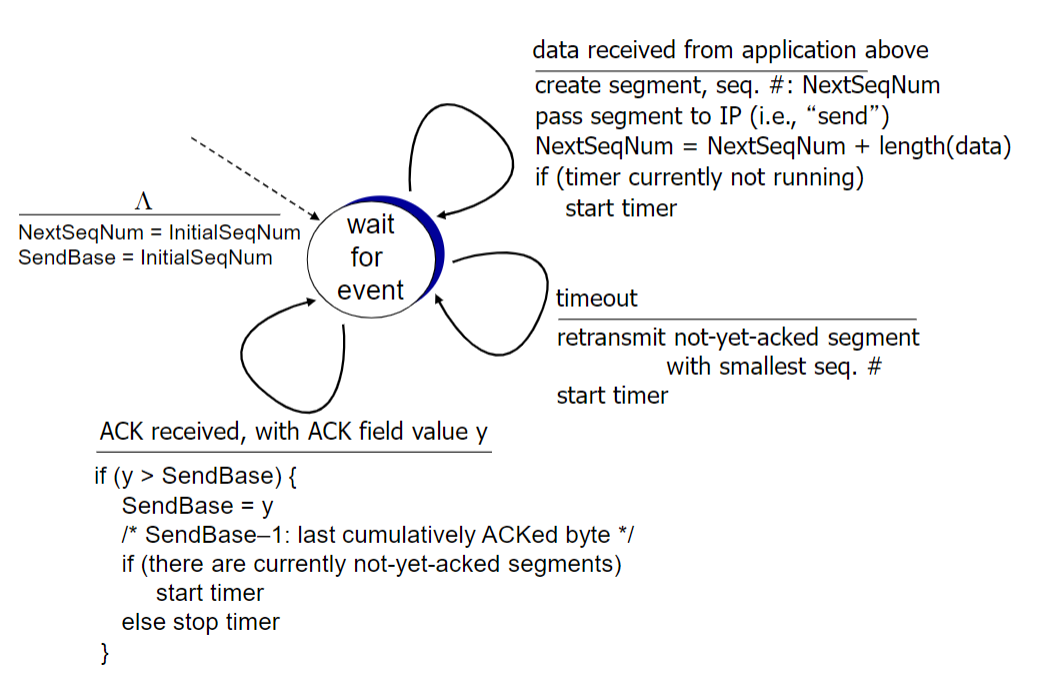
\includegraphics[width=0.65\linewidth, align=c]{images/TCP_sender_simple.PNG}
\end{figure}

\paragraph{Fast retransmit}
\begin{itemize}
    \item If sender receives 3 duplicate (extra) ACKs for same data, it will resend unACKed segment with smallest \texttt{seq\_num}.
\end{itemize}

\subsection{Other Reliable Data Transfer (RDT) Protocols}
\subsubsection{Go-Back-N (GBN)}
\begin{itemize}
    \item Requirement for k-bit \texttt{seq\_num} in packet header: $2^k > N$
    \item Receiver window size: 1 (\texttt{expected\_seq\_num}).
    \item Relationship among \texttt{expected\_seq\_num}, \texttt{send\_base}, \texttt{next\_seq\_num}:
    \begin{itemize}[label=$\circ$]
        \item \texttt{send\_base} $\leq$ \texttt{next\_seq\_num} $\leq$ \texttt{expected\_seq\_num}
    \end{itemize} 
\end{itemize}

\subsubsection{Selective Repeat (SR)}
\texttt{rcv\_base} = \texttt{next\_seq\_num} if all packets up to \texttt{next\_seq\_num} are received

\begin{itemize}
    \item Requirement for k-bit \texttt{seq\_num} in packet header : $2^k > 2N$
    \item Receiver window size: 1 (\texttt{expected\_seq\_num}).
    \item Relationship among \texttt{expected\_seq\_num}, \texttt{send\_base}, \texttt{next\_seq\_num}:
    \begin{itemize}[label=$\circ$]
    \item \texttt{send\_base} $<$ \texttt{next\_seq\_num} $<$ \texttt{expected\_seq\_num}
    \end{itemize}
\end{itemize}

\newpage
\section{Lecture 10: Congestion Control}
\subsection{Principles of Flow Control}
\begin{itemize}
    \item Receiver controls sender so the sender won't overflow receiver's buffer by transmitting too much/too fast
    \begin{itemize}[label=$\circ$]
        \item Application may remove data from TCP socket buffers
    \end{itemize}
    \item Receiver includes a \texttt{rwnd} (receiver window) value in TCP header of receiver-to-sender segments
    \begin{itemize}[label=$\circ$]
        \item \texttt{RcvBuffer}
    \end{itemize}
\end{itemize}

\subsection{Principles of Congestion Control}
\begin{itemize}
    \item Congestion Control $\neq$ Flow Control!
    \item Mainfestations
    \begin{itemize}[label=$\circ$]
        \item Buffer Overflow at Routers: Lost Packets
        \item Queueing in Router buffers: Long Delay
    \end{itemize}
\end{itemize}
\noindent When packets are lost, any upstream transmission capacity used for that packet is wasted.

\subsubsection{Scenario 1: One Router w/ Infinite Buffers}
\begin{itemize}
    \item Assuming no retransmission
\end{itemize}

\subsubsection{One Router w/ Finite Buffers}
Assumptions for idealized case
\begin{itemize}
    \item Sender knows when router buffers available
    \item Sender sends only when router buffers available
\end{itemize}
Transfer rates
\begin{itemize}
    \item $\lambda_{\text{in}} = \lambda_{\text{out}}$: Application-layer input = output
    \item $\lambda_{\text{in}}' \geq \lambda_{\text{in}}$: Transport-layer input includes retransmissions
\end{itemize}

\subsubsection{TCP Congestion Controls}
\noindent\textbf{Increase sender's transmission rate until loss occurs}
\begin{itemize}
    \item Additive Increase: Increase cwnd (congestion window) by 1 MSS every RTT until loss detected
    \item Multiplicate Increase: Reduce cwnd in half after loss
\end{itemize}

\newpage
\section{Lecture 11: TCP Wrapup}
\subsection{TCP Congestion Control}
A summary code for the sections discussed below:
\begin{python}
    cwnd = MSS
    while connected:
    if time < slow_start_duration:
        cwnd *= 2
        if receive_ACK: 
        cwnd += MSS
    else: # congestion-avoidance state
        if receive_ACK:
        cwnd += MSS*(MSS/cwnd)
\end{python}
\begin{figure}[H]
    \centering
    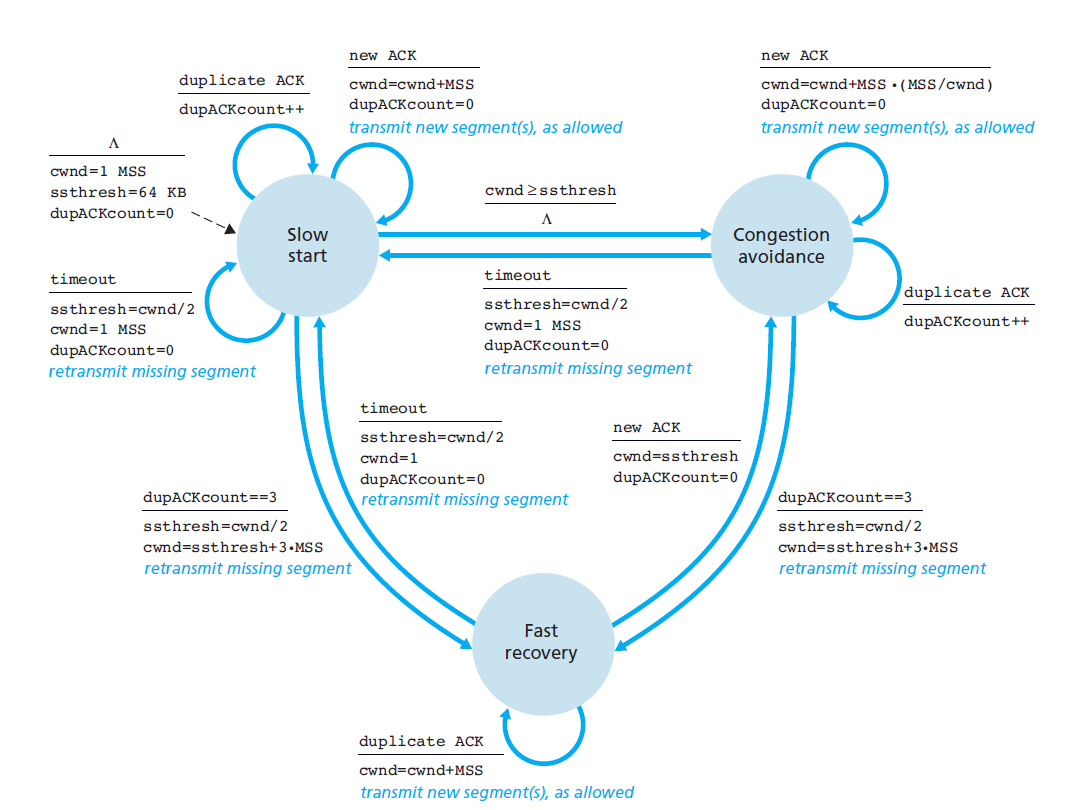
\includegraphics[width=0.9\linewidth, align=c]{images/TCPCongestionControl.PNG}
\end{figure}

\subsubsection{Start Connection: Slow Start}
When connection begins, increase rate exponentially until first loss event. (Initial rate is slow but ramps up very fast)
\begin{enumerate}
    \item Initial \texttt{cwnd}: 1 MSS (maximum segment size)
    \item Double \texttt{cwnd} every RTT
    \begin{itemize}
        \item It is doubled with the formula: $cwnd = cwnd + MSS * \displaystyle\frac{cwnd}{mss}$
    \end{itemize}
    \item Increment \texttt{cwnd} for every ACK received
\end{enumerate}

\subsubsection{Congestion-avoidance state}
Window grows exponentially in \textbf{slow start} to threshold, then grows linearly during the congestion-avoidance (CA) state. 
\begin{itemize}
    \item The inexponential increase is switched to linear when \texttt{cwnd} gets to half of its value before timeout.
    \item On loss event, \texttt{ssthresh}=0.5\texttt{*cwnd} before loss event.
\end{itemize}
In the CA state, the congestion window is increased by $\displaystyle\frac{1}{k}$.
\begin{itemize}
    \item where $k$ = $\displaystyle\frac{cwnd}{mss}$
\end{itemize}

\subsubsection{Explicit Congestion Notification (ECN)}
\paragraph{Network-assisted congestion control}
\begin{itemize}
    \item 2 bits in IP header (ToS field) marked by network router to indicate congestion
    \item Receiver sets ECE bit on ACK to notify sender of congestion
\end{itemize}

\subsubsection{Calculating TCP Throughput}
Ignoring slow start and assuming there is always data to send,
$$\text{TCP Throughput} = \frac{3}{4}*\frac{W}{RTT}$$
\begin{itemize}
    \item where $W$: window size in bytes where loss occurs
\end{itemize}
\begin{figure}[H]
    \centering
    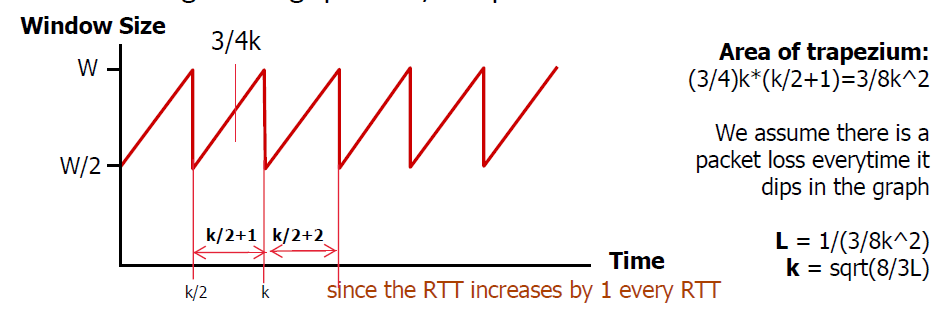
\includegraphics[width=0.7\linewidth, align=c]{images/tcp_throughput.PNG}
\end{figure}

\paragraph{Calculating Segment Loss Probability, L}\mbox{}\\
e.g. given 1500 byte segments, 100ms RTT, 10Gbps throughput, requires average 83,333 in-flight segments
\begin{align*}
    10^7 &=  \frac{1.22\times1500}{100\times10^{-3}\times\sqrt{L}}\\
    L &= 2\times 10^{-10}
\end{align*}

\newpage
\subsubsection{TCP Fairness}
\begin{itemize}
    \item Goal: For $n$ TCP sessions sharing same bottleneck link of bandwidth $R$, each should have $\displaystyle\frac{R}{K}$ rate.
    \item Implementation via Additive Increase and Multiplicate Decrease
\end{itemize}
\begin{figure}[H]
    \centering
    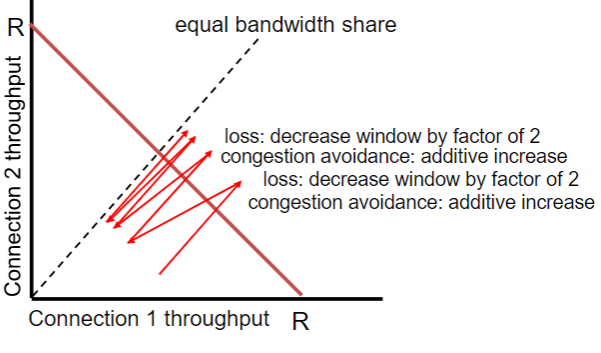
\includegraphics[width=0.7\linewidth, align=c]{images/tcp_fairness.PNG}
\end{figure}

\end{document}